\chapter{CMS}


\section{Proxy}
Ein Proxy ist ein Stellvertreter oder auch Vermittler. Oft wird die Funktionalität des Proxy sowie die des \textbf{Cache} in einem Server/Device angeboten. Der Cache speichert die Antwort des Client-Requests. Damit wird bei einem späteren Request eines Clients der Zugriff auf die Ressource ins Internet vermieden. Wir unterscheiden zwei Proxy-Arten:

\begin{description}
	\item[Forward Proxy:] Versteckt die Identität des Client vor dem Server. Der Client ruft einen Server über einen Proxy auf, dabei weiss der Server nicht, wer der konkrete Client ist.
	\item[Reverse Proxy:] Versteckt die Identität des Servers vor dem Client.  Dieser nimmt die Anfragen im Internet entgegen und leitet diese an andere Server im internen Netzwerk weiter. Der Anfragende verbindet sich nur mit dem Proxy, das interne Netzwerk muss nicht bekannt sein.
\end{description}

\begin{figure}[h!]
	\centering
	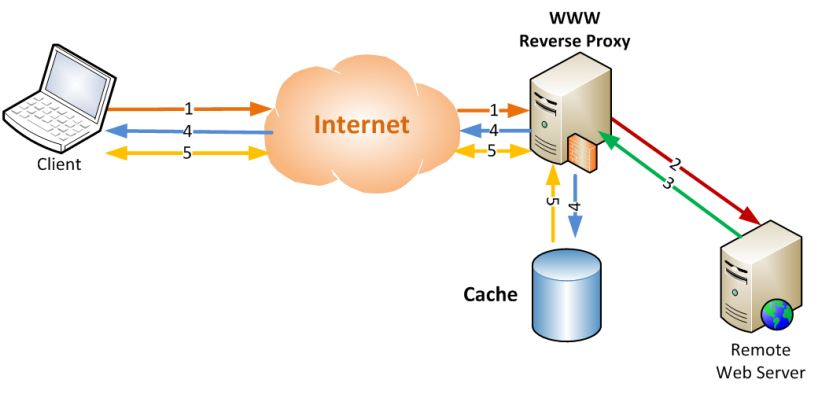
\includegraphics[width=0.7\linewidth]{fig/cms-reverse-proxy-cache}
	\caption{Reverse Proxy und Cache in Action}
	\label{fig:cms-reverse-proxy-cache}
\end{figure}

\section{Web Application Firewall}
Eine Web Application Firewall (WAF) werden oft auch \emph{Deep Packet Inspection Firewall} genannt und geht im Grundsatz auf zwei Fragen ein: Wer jemand ist und was er tut. WAFs suchen gezielt nach Signaturen einer Attacke oder nach abnormalen Verhalten. WAFs können als Reverse Proxy auf dem Weg zum Webserver installiert werden. Ein wesentlicher Vorteil ist, dass man bestehende Web-Applikationen \textbf{nachträglich absichern} kann, falls diese \textbf{keinen ausreichenden Schutz} gewähren. So muss man die Web-Applikation nicht umprogrammieren. Airlock ist eine sehr gute WAF, welche auch Loadbalancing und Reverse Proxy kann. Gemäss Infanger sogar die beste und ein Produkt aus der Schweiz. Auf dem Markt existieren nur 5 WAFs, welche brauchbar sind.

\section{Loadbalancer}
Leitet die Anfrage an einen 'freien' Server weiter und muss dafür kontinuierlich die Serverlasten messen. Das führt dazu, dass der Loadbalancer Request-Queues verwalten muss. Dies wird oft mit einem Reverse Proxy oder WAF kombiniert.

\subsection{DNS Round Robin}
Ein simple Idee wäre, dass gleich der DNS-Dienst eine Lastverteilung durchführt. Wenn ein Client X kommt, dann bekommt er die IP des Server A, wenn Client Y kommt dann bekommt er die IP des Server B. Aber das geht nur bedingt, da im DNS Bereich viel gecacht wird und nicht für jeden Request der DNS angefragt wird. Grosse Firmen benutzen dies schon auch. Ich denke, dass es beispielsweise Sinn machen kann, dass Netflix bei Anfragen aus Europa, dann die europäischen Netflix-Server zurückliefert und Anfragen in Amerika die entsprechenden Server dort.

\subsection{DNS und Reverse Proxy}
Über den DNS wird die IP des Reverse Proxy mitgeteilt. Das Load Balancing wird anschliessend vom Reverse Proxy vollständig umgesetzt.



% Themen
% Aufbau WCMS Systeme
% n-tier Architektur
% Server-Typen
% Performance-Indikatoren
% Session-Handling
% vertical und horizontal Scaling/Partitioning
% Netzwerk-Infrastrukturen (Sicherheit-Loadbalancing-SPOF)
% done Reverse Proxy: Funktionsweise und Verwendungszweck bzw. Einsatzmöglichkeiten.

% Dokumente: 
% 03a.CMS-Systeme.pdf
% done 03b.ReverseProxySysteme.pdf (ausser Airlock Setup)
% 03c.building-scalable-architecture.pdf (grundsätzliche Prinzipien der Skalierung aber ohne DB-interne und SAN Aspekte, bis Seite 30)